\documentclass[12pt,fleqn]{article}
\usepackage{a4}
\usepackage{graphicx}
\usepackage{psfrag}
\usepackage{amsmath}                     % \boldsymbol{#1}
\usepackage{amssymb}
%\usepackage{hangcaption}
%\usepackage{Styles/pstricks}
%\usepackage{Styles/pst-node}
\usepackage{Styles/fancyheadings}
\usepackage{tocloft}
%-----Tex width---------------------------------
\textwidth 16cm

%-----Line spacing-------------------------------
\renewcommand{\baselinestretch}{1.5}     % 1,1-zeilig

%---------Add dots in TOC-----------------------
\renewcommand{\cftsecleader}{\cftdotfill{\cftdotsep}}

%------Paragraph indention-------------------------------
\setlength{\parskip}{1.5ex plus0.5ex minus0.5ex}

%-----Prevent indent----------------------
\setlength{\parindent}{0em}

%-----Richtiger Abstand fur Einheiten-------------
\def\Unit{\hspace{0.25em}}

%-----Definition of the header--------------------
\pagestyle{fancyplain}
\renewcommand{\sectionmark}[1]{\markboth{Chapter~\thesection.~#1}{#1}}
\renewcommand{\subsectionmark}[1]{\markright{\thesubsection\ #1}}
\rhead[\fancyplain{}{\leftmark}]%
{\fancyplain{\thepage}{\thepage}} \cfoot{} \plainheadrulewidth
0.4pt
%% Otherwise: Overfull \vbox-Warning against fancyheadings-pacakage
%%  idea of: nic@minster.york.ac.uk (Nick Cropper)
\makeatletter
\ifcase \@ptsize \relax % 10pt
  \addtolength{\headheight}{1\p@}
\or % 11pt
  \addtolength{\headheight}{2\p@}
\or % 12pt
  \addtolength{\headheight}{3\p@}
\fi \makeatother

%-----Equations / Figures / Tables numbering according to \ sections
\makeatletter
\renewcommand\theequation{\thesection.\arabic{equation}}
\renewcommand\thefigure{\thesection.\arabic{figure}}
\renewcommand\thetable{\thesection.\arabic{table}}
\@addtoreset{equation}{section} \@addtoreset{figure}{section}
\@addtoreset{table}{section} \makeatother

%-----Useful abbreviations----------------------
\newcommand{\mr}{\mathrm}
%%\newcommand{\bs}[1]{\mbox{$\boldsymbol{#1}$}}
\newcommand{\degree}[1]{\mbox{$#1^\circ$}}

%\renewcommand{\figurename}{Bild}

%------Bibliography style-----------------------
\bibliographystyle{IEEEtran}

%-----Aufzaehlunstiefe im Literaturverzeichnis---------------
\setcounter{tocdepth}{3}

\begin{document}
\pagenumbering{Roman}
\begin{titlepage}
  \begin{center}
      \vspace*{-4.0cm}
    \begin{figure}[!h]
\centering

\includegraphics[width=0.3\linewidth]{Figures/JKUAT_logo}
%\caption{}
\label{fig:jomologo}
\end{figure}
   \large{Jomo Kenyatta University of Agriculture and Technology}\\
    \large{College of Engineering and Technology}\\
    \large{School of Mechanical, Materials, and Manufacturing Engineering}\\
   \large{Department of Mechatronic Engineering}\\

    ------------------------------------------------------------------------------------------------\\[1.0cm]
    \LARGE{\textbf{Development of a 6 DOF Stewart platform
        Force Balance for a Low Speed Wind Tunnel}}\\[0.6cm]
    \LARGE{\textbf{Final year proposal (FYP 18-10)
            }}\\[1.5cm]
    %\large{by}\\[0.6cm

    \vspace{0.5cm}
    \large{\textbf{Sammy Kerata Oina (ENM221-0089/2017)
            }}\\
     \large{\textbf{Earl Spencer Mogire~(ENM221-0074/2017)
            }}\\[1.0cm]
%     \large{\textbf{Supervisors}}\\
%    \large{Dr.-Ing.~Jackson G. Njiri}\\
%    \large{Prof. George N. Nyakoe}\\
%    \large{\ldots}    \\[0.2cm]\vfill
    \large{\small{\today}}\\
    ------------------------------------------------------------------------------------------------\\[1.5cm]
  \end{center}
\end{titlepage}
%
%\pagenumbering{gobble}% Remove page numbers (and reset to 1)

\addcontentsline{toc}{section}{Declaration}
\section*{Declaration}

We hereby declare that the work contained in this report is original; researched and documented by the undersigned students. It has not been used or presented elsewhere in any form for award of any academic qualification or otherwise. Any material obtained from other parties have been duly acknowledged. We have ensured that no violation of copyright or intellectual property rights have been committed.
\begin{enumerate}
	\item Sammy Kerata Oina\vspace*{.2cm}\\
	Signature\ldots\ldots\ldots\ldots\ldots\ldots\ldots\ldots\ldots\ldots Date\ldots\ldots\ldots\ldots\ldots\ldots\ldots\ldots\ldots\ldots
	\item Earl Spencer Mogire\vspace*{.2cm}\\
	Signature\ldots\ldots\ldots\ldots\ldots\ldots\ldots\ldots\ldots\ldots Date\ldots\ldots\ldots\ldots\ldots\ldots\ldots\ldots\ldots\ldots
\end{enumerate}

\vspace*{.5cm}
Approved by supervisors:
\begin{enumerate}
	\item Ir. Anthony K. Muchiri \vspace*{.2cm}\\
	Signature\ldots\ldots\ldots\ldots\ldots\ldots\ldots\ldots\ldots\ldots Date\ldots\ldots\ldots\ldots\ldots\ldots\ldots\ldots\ldots\ldots
	%\item Prof. George N. Nyakoe\vspace*{.2cm}\\
	%Signature\ldots\ldots\ldots\ldots\ldots\ldots\ldots\ldots\ldots\ldots Date\ldots\ldots\ldots\ldots\ldots\ldots\ldots\ldots\ldots\ldots
	\item Ms. Maurine Andanje\vspace*{.2cm}\\
	Signature\ldots\ldots\ldots\ldots\ldots\ldots\ldots\ldots\ldots\ldots Date\ldots\ldots\ldots\ldots\ldots\ldots\ldots\ldots\ldots\ldots
\end{enumerate}



\clearpage
\addcontentsline{toc}{section}{Table of Contents}
\tableofcontents
\clearpage
\addcontentsline{toc}{section}{List of Figures}
{%
\let\oldnumberline\numberline%
\renewcommand{\numberline}{\figurename~\oldnumberline}%
\listoffigures
\clearpage
\addcontentsline{toc}{section}{List of Tables}
\listoftables
\newpage
\clearpage
\addcontentsline{toc}{section}{List of Abbreviations}
\clearpage
\newpage

\newpage
\paragraph{Nomenclature}
\begin{itemize}
\item DAQA - Data Acquisition System
\item DOF - Degrees of Freedom
\item JKUAT - Jomo Kenyatta University of Agriculture and Technology
\item NASA - National Space Agency
\item SPI - Serial Peripheral Interface
\item B - coordinate system defined at center of base plate
\item $\vec{b}_i$ - position of ith connection point at base with respect to B
\item $\hat{I}_i$ - Unit vector along the ith leg
\item $\vec{F}_e$ - external force applied to platform
\item $\vec{M}_e$ - external momment applied to platform
\item $f_i$ - force exterted on ith leg due $F_e, M_e$
\item $F$ - vector of leg forces
\item $H$ - transformation matrix which related measured forces and applied forces 
\end{itemize}
\pagebreak
\addcontentsline{toc}{section}{Abstract}

\section*{Abstract}
\label{sec:Abstract}
Obtaining and simulating the aerodynamic performance of items in a wind tunnel is a
significant and important part in the development of vehicles, aircraft and other machines
that require aerodynamic performance evaluation. Due to the complex maneuvers that may require simulation, there is a need for dynamic positioning of the model of the object in the wind tunnel. As a result, the proposal for a Stewart platform to replicate these complex maneuvers during wind tunnel tests as well as to position the model to obtain the required data.

This project will look into the modeling, simulation and development of a Stewart
platform based force balance for a low speed wind tunnel. The project will utilize
MATLAB/Simulink for modeling and simulation as well as Autodesk Inventor for the mechanical
design. A robust control system will also be developed for the Stewart platform.
Finally, models will be developed and tested in a wind tunnel to evaluate the performance
of the platform. The force balance and platform should be able to position the test
item and measure forces as well as calculate the aerodynamic coefficients using a bespoke computer program.





\clearpage
\pagenumbering{arabic}
  \section{Introduction}
\subsection{Background}
\subsubsection{Stewart Platform}
\subparagraph*{Description of Mechanism}
\paragraph{}A stewart platform is a platform with six degrees of freedom (DOF). The six-degrees-of-motion platform is capable of moving in three linear directions and
three angular directions singly or in any combination.
It comprises a triangular/rectangular/circular plane called the platform, of which each of the corners (for triangualar platform in this case) is connected through a three-axis joint to one of three legs. This is shown in Fig.1.1.
\begin{figure}[!h]
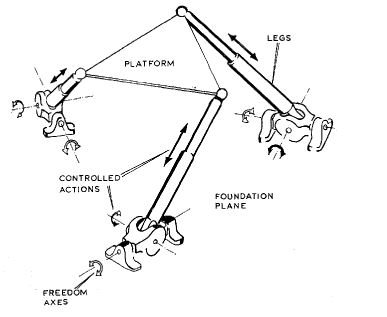
\includegraphics{Figures/Fig1}
\caption{General arrangement}
\end{figure}
\paragraph{}Each leg is connected to the ground by a two-axis joint where: One of these axes is
normal to the leg and is provided with a means for control wheareas, the other axis is normal to the first and is not provided with a means for control.
Each leg also has controllable means for extending its length. These control means include:
\begin{enumerate}
\item Use of two hydraulic jacks
\item Screw Jacks
\item Rotary actuator
\item Levers
\item Linear co-ordinate control
\item Strength
\end{enumerate}
\paragraph{}These shall be discussed in detail at a later stage.

\subparagraph{Application}
\paragraph{}The six DOF Stewart Platform provides an elegant design for simulating flight conditions which finds applications in the safe training of pilots. The mechanism differs from other simulators in that it has no fixed axes relative to the ground, and therefore within the limits of amplitude of the design it can truly simulate the conditions of banking by carrying the simulation of control surfaces into the axes of the new attitude.

\subsubsection{Force Balance}
\subsubsection{Wind Tunnel}
\paragraph{}
A wind tunnel is a large tube with air moving inside. This movement of air is usually done by powerful fans. The tunnel is used to copy the actions of an object in flight. The first wind tunnel was built by
Francis Wenham in 1871. However, it was the Wright Brothers who were the first to show the value of the wind tunnel in aerodynamic design with their 1902 wind tunnel.  The Wright Brothers’ wind tunnel was largely made of wood, with a glass window on the top to look down through and see the force balance, from which the
lift and drag forces could be read. The wind tunnel was powered by a fan driven off a natural gas fueled engine. Their tunnel was square of 16" by 16"(about 407mm by 407mm), and 6 foot long (about 1829mm), with a maximum test speed of 35 mph (about 56 km/h).
\begin{figure}[!h]
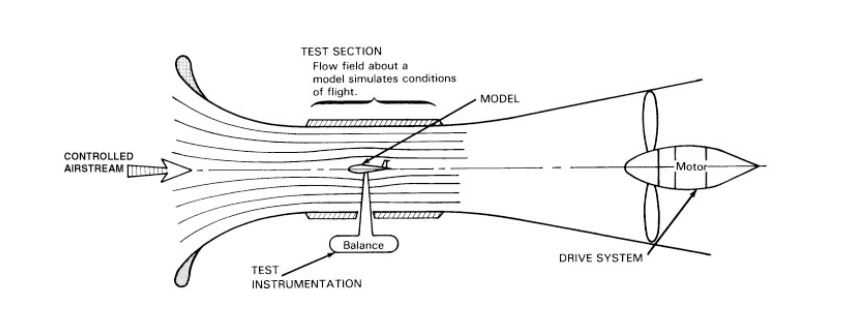
\includegraphics{Figures/Fig2}
\caption{Diagram of a typical wind tunnel}
\end{figure}
\paragraph{}
Later in the early 20th century in Europe, the main users of wind tunnels were Gustave Eiffel in France and Ludwig Prandtl in Germany. Prandtl built the first closed circuit wind tunnel in 1908. By the 1940’s supersonic wind tunnels were in use. In 1972 a cryogenic wind tunnel was built at NASA Langley by injecting liquid nitrogen into the wind tunnel to cool the gas. This lowered the viscosity and increased the Reynolds number, and this tunnel had the capability to match Reynolds and Mach numbers simultaneously up to Mach 1.2. 
\paragraph{}Today the largest wind tunnel in the world is the National Full-Scale Aerodynamics Complex at NASA's Ames Research Center, which has a test section of cross section 80 ft by 100 ft (24 m x 31 m). The types of instruments in common use in wind tunnels include boundary layer rakes, tufts, pitot tubes, pressure sensitive paint, smoke, and static pressure taps.
\begin{figure}[!h]
\hfill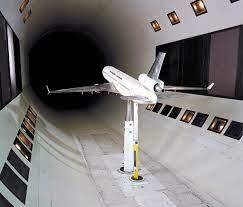
\includegraphics{Figures/Fig3}\hspace*{\hfill}
\caption{NASA wind tunnels used to test new airplane designs}
\end{figure}

\paragraph{}NASA uses wind tunnels to test scale models of aircraft and spacecraft. Wind tunnels help NASA to test ideas of making airplanes better and safer. They are also used to help engineers in designing spacecraft that will work in other planets such as mars - the wind tunnel can be used to simulate objects in an atmosphere that's thinner than ours i.e. an atmosphere that's exactly like the Martian atmosphere. NASA has wind tunnels of different types and sizes. Some are low-speed wind tunnels, others are hypersonic i.e. they are made to carry out tests at 4,000 mph (6437 kph).
\begin{figure}[!h]
\hfill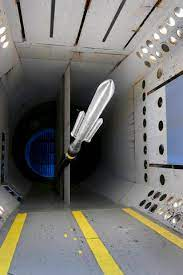
\includegraphics{Figures/Fig4}\hspace*{\hfill}
\caption{NASA wind tunnels used to test the design of heavy-lift rocket}
\end{figure}
\paragraph{}Wind tunnels are used to measure the aerodynamic forces on airplanes, wings, cars, trucks, bridges, and buildings, they can also be used to measure the
aerodynamic forces on sports balls, partially open valves, and anything else that can be mounted on the mounting sting. Wind tunnels are an effective tool used by engineers in determining the various aerodynamic loads due to movement of these vessels during the development process.
For wind tunnel testing with scale models to be applicable to the aerodynamics of the full-scale test object, conditions of dynamic similarity must be met.
\paragraph{}Wind tunnel testing is not cheap i.e. both to buid and to use. While a crude wind tunnel can be constructed relatively cheaply from a large fan and
sheet metal, our project will be limited to development of the six-degrees-of-freedom Stewart Platform and Force balance. We will use the low speed wind tunnel that is currently available at ?????
\subsection{Problem statement}
(Insert your content)
\subsection{Objectives}
(Insert your content)
\subsection{Justification of the study}
\paragraph{}Additive manufacturing offers the ability to produce intricate products and parts with lower development costs, shorter lead times, less energy consumed during manufacturing as well as less material waste. This method can be used to manufacture delicate components such as the bipolar plates with elimination of the risks involved such as breakage of brittle Graphene material during production.     
\paragraph{}Precise control of reactant flow and pressure, stack temperature, and membrane humidity will increase the fuel cell’s robustness as well as efficiency.
\paragraph{}The goal of this research is to develop physic-based dynamic models of fuel cell systems and fuel processor systems and then apply multivariable control techniques to study their behavior. The analysis will give insight into the control design limitations and provide guidelines for the necessary controller structure and system re-design.

  \clearpage
  \section{Literature Review}
\subsection{Stewart Platform}
Parallel link manipulators have become an important area of research due to their: precision, rigidity and high-load-to-weight ratio. These manipulators find practical applications in flight simulators, precise machining and applications that require disturbance isolation. \cite{iqbal_dynamic_2008}. The Stewart platform is an example of a parallel manipulator.

A Stewart platform is a parallel manipulator that provides six-degree-of-freedom (DOF) i.e. roll, pitch, yaw, surge, sway and heave, and can be controlled in all these freedoms simultaneously. The platform consists six variable-length electro-mechanical actuators connecting a top plate to a base plate with spherical joints.

The platform is able to move in three angular directions and in three linear directions, singly or in any combination \cite{stewart1965platform}. Angular and translational motion of the top plate with
respect to the base plate is achieved by reducing or extending the actuator lengths. For the top plate to follow the desired trajectory with high frequency, there has to be proper coordination of the actuator lengths \cite{iqbal_dynamic_2008}.

Each leg of the mechanism is connected to the ground by a two-axis joint where: One of these axes is
normal to the leg and is provided with a means for control whereas, the other axis is normal to the first and is not provided with a means for control.
Each leg also has controllable means for extending its length. These control means include:
\begin{enumerate}
\item Use of hydraulic jacks.
\item Screw jacks - This gives give the advantage of
a longer stroke for a given size.
\item Rotary actuator - a hydraulic rotary actuator or an electric motor. Whereas this would reduce the number of foundation fixings, the remaining jack would still be subjected to a greater bending moment.
\item Levers - this increases the extending leg amplitude by using an articulated leg.
\item Linear co-ordinate control - this arrangement provides rigidity due to the true triangulation of
the whole system. There will be no bending moments in any of the members apart from the possibility of those due to strut eccentric loading. 
\end{enumerate}
\begin{center}
	\begin{figure}[!h]
	\centering
	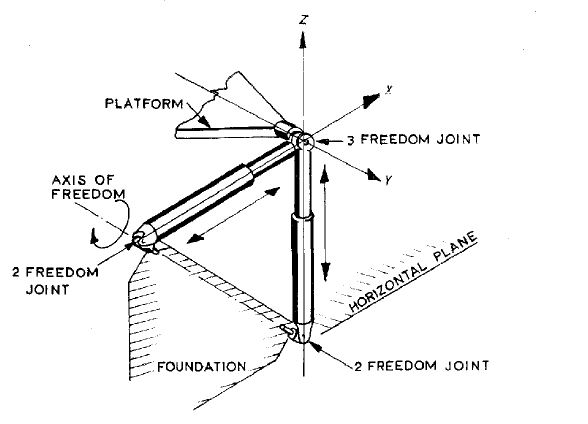
\includegraphics[width=0.6\linewidth]{Figures/Fig11}
	\caption{Linear co-ordinate control}
	\end{figure}
\end{center}

Stewart platforms that use screw jacks driven by electric motors as leg actuators have the advantage of being light and easy to control. Velocity and position control for these platforms can be done using shaft encoders and tachometers. A ball screw is used to minimize friction in a screw drive and backlash in the ball screw can be eliminated by use of double nuts preloaded with spring washers \cite{fichter1986stewart}.

In order to control the platform in the required direction, a program involving linear or angular accelerations or a combination of both is necessary so that signals can be given to the various legs in accordance with the input requirements. The six inputs to the Stewart platform in terms of torque are calculated by the controller and the outputs of the Stewart platform are the upper plate's angular and translational positions sensed by highly precise sensors or estimated by the motor's encoders \cite{iqbal_dynamic_2008}.

Further, as concerns the control aspect, in recent years many researchers have worked on robust controllers for the Stewart platform. Some of these works include:
\begin{enumerate}
\item A Lyapunov based approach for designing robust PD controller was proposed in presence of uncertainties 
\cite{kang1996robust}.
\item The model based sliding mode control with perturbation 
\cite{kang1996robust}.
\item Robust tracking control design in the presence of time varying
uncertainties 
\cite{kim1998high}.
\item Tracking errors drive to zero asymptotically with help of sliding mode
controller design 
\cite{huang2004sliding}.
\item A simple way to calculate control law using sliding-mode technique 
\cite{iqbal2006direct}.
\end{enumerate}

\subsubsection{Wind Tunnel}
A wind tunnel is a large tube with air moving inside. This movement of air is usually done by powerful fans. 

The first wind tunnel was built by Francis Wenham in 1871. However, it was the Wright Brothers who were the first to show the value of the wind tunnel in aerodynamic design with their 1902 wind tunnel.  The Wright Brothers’ wind tunnel was largely made of wood, with a glass window on the top to look down through and see the force balance, from which the
lift and drag forces could be read. The wind tunnel was powered by a fan driven off a natural gas fueled engine. Their tunnel was square of 16" by 16"(about 407mm by 407mm), and 6 foot long (about 1829mm), with a maximum test speed of 35 mph (about 56 km/h).
\begin{center}
	\begin{figure}[!h]
	\centering
	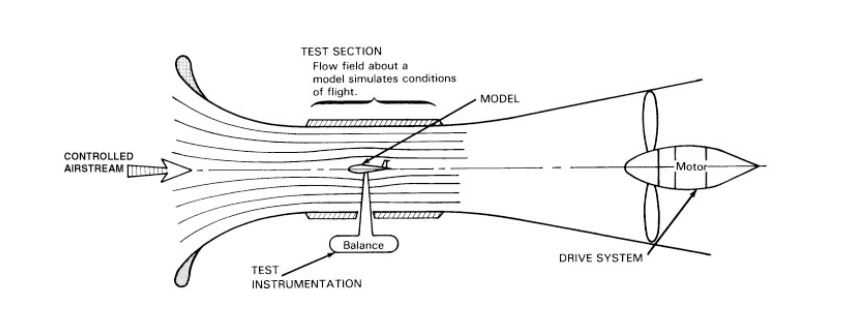
\includegraphics[width=0.75\linewidth]{Figures/Fig2}
	\caption{Diagram of a typical wind tunnel}
	\end{figure}
\end{center}

Later in the early 20th century in Europe, the main users of wind tunnels were Gustave Eiffel in France and Ludwig Prandtl in Germany. Prandtl built the first closed circuit wind tunnel in 1908. Closed circuit wind tunnels are characterized by the recirculation of the airflow with very minimal exchange with the exterior. Open circuit wind tunnels on the other hand, have an airflow that follows a straight path and flows to the contracted zone where the test section is located and then passes through a diffuser, a fan section and an exhaust.

By the 1940’s supersonic wind tunnels were in use. In 1972 a cryogenic wind tunnel was built at NASA Langley by injecting liquid nitrogen into the wind tunnel to cool the gas. This lowered the viscosity and increased the Reynolds number, and this tunnel had the capability to match Reynolds and Mach numbers simultaneously up to Mach 1.2
\cite{fernandes_design_nodate}.

Today the largest wind tunnel in the world is the National Full-Scale Aerodynamics Complex at NASA's Ames Research Center, which has a test section of cross-section 80 ft by 100 ft (24 m x 31 m). The types of instruments in common use in wind tunnels include boundary layer rakes, tufts, pitot tubes, pressure sensitive paint, smoke, and static pressure taps.
\begin{center}
\begin{figure}[!h]
	\centering
	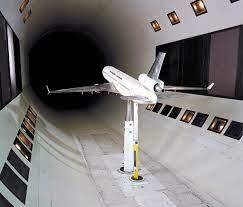
\includegraphics{Figures/Fig3}
	\caption{NASA wind tunnels used to test new airplane designs}
\end{figure}
\end{center}

NASA uses wind tunnels to test scale models of aircraft and spacecraft. Wind tunnels help NASA to test ideas of making airplanes better and safer. They are also used to help engineers in designing spacecraft that will work in other planets such as mars - the wind tunnel can be used to simulate objects in an atmosphere that's thinner than ours e.g. an atmosphere that's exactly like the Martian atmosphere. NASA has wind tunnels of different types and sizes. Some are low-speed wind tunnels, others are hypersonic i.e. they are made to carry out tests at 4,000 mph (6437 kph).
\begin{center}
     %&\vspace*{-4.0cm}
    \begin{figure}[!h]
\centering
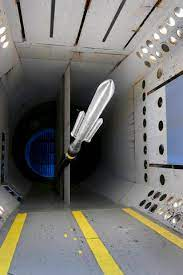
\includegraphics{Figures/Fig4}
\caption{NASA wind tunnels used to test the design of heavy-lift rocket}
\end{figure}
\end{center}
\subsection{Force Balances}
For wind tunnel applications, the wind axes is used as the reference frame. Where, X axis points to the accelerated air; Z axis points downward and; Y axis points to the right in the direction of the wind. In the reference frame above, lift is in the negative z-direction, drag in the negative x-direction and, side force in the negative y-direction.

Moment components on the x,y,z axes are rolling moment, pitching moment and yawing moment respectively. A three-component force balance can be considered to measure the lift, drag and pitch (angle of attack).

Force balances can be external or internal. In external force balances the test section lies outside of the wind tunnel test section, whereas in internal force balances the balance is inside the model itself connecting the model to the support structure.

Several different types of external force balances are available for wind tunnel use
\cite{morris_force_2010}:
\begin{enumerate}
\item Wire
\item Platform
\item Yoke
\item Pyramidal
\end{enumerate}
\begin{center}
	\begin{figure}[!h]
	\centering
	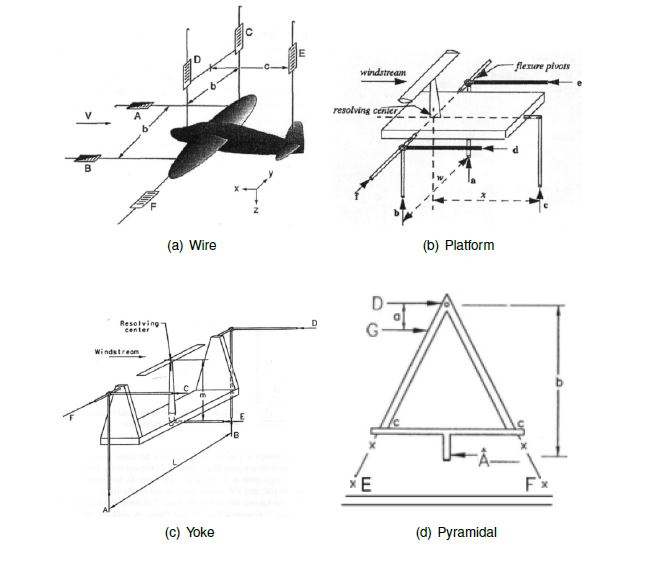
\includegraphics{Figures/Fig6}
	\caption{Typical configurations for external force balances}
	\end{figure}
\end{center}
In the wire balance, the model under testing is suspended by wires each connected to an extensometer (a sensor that produces an electrical output when submitted to a load and deforms). The shortcoming of the wire balance is the large tare drag caused by the wires which is difficult to quantify. They are also not robust nor versatile enough compared with the other alternatives. 

The platform balance is relatively easy to construct, assemble and instrument. However, for this balance, forces and torques are coupled and the balance resolving center does not coincide with the center of the tunnel.
 
In the yoke balance configuration, forces and torques are coupled and the balance resolving center coincides with the center of the tunnel. This configuration, however, presents some structural deflections due to the large span of the measuring and support arms.

The pyramidal balance configuration is a further improvement of the yoke balance in order to overcome the shortcomings of the other balances. It is capable of measuring six components of forces and
torques separately and without coupling,provided that the balance is well assembled and calibrated.

The different kinds of internal balances can be made based on:
\begin{enumerate}
\item The type of transducer i.e. strain gauge or piezoelectric balance.
\item Shape i.e. box balance and sting balance
\end{enumerate} 
\begin{center}
	\begin{figure}[!h]
	\centering
	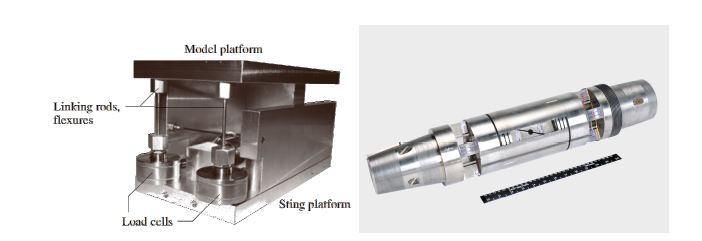
\includegraphics{Figures/Fig7}
	\caption{Typical configurations for internal force balances. \textit{Left to right:} Box balance and sting balance.}
	\end{figure}
\end{center}
The box balance presents a cubic shape and can either be made of a solid piece of material or from assembled parts. In this configuation, the loads are transferred from the top to the bottom. The sting balance presents a cylindrical shape and the loads are transferred from one end to the other in the longitudinal direction. It can be used to measure forces or torques.

The advantage of internal force balances is that they minimize the interference caused by the supporting bars in the flow.
\subsection{Sensors}
\subsubsection{Load Sensors}
Several methods can be used to measure forces and torques in a force balance. These methods can be generally grouped into two:
\begin{enumerate}
\item Hydraulic measuring techniques.
\item Electric measurement techniques.
\end{enumerate}
Electric measurement techniques are preferred for Force balance applications. One such electric measurement device is the strain gauge. A strain gauge is an electromechanical device whose electrical resistance changes linearly with the strain in the component.

Metal foil strain gauges are widely used. This type of strain gauge provide more precise strain values than wire strain gauges. However, since the relative changes on electric resistance of the strain gauge are so small, it is necessary to develop an effective method to measure them because each strain gauge would require extremely accurate signal measurements. The solution is to have a set of strain gauges coupled in order to minimize the required accuracy, forming a force transducer i.e. the \textit{Wheatstone bridge}.
\begin{center}
		\begin{figure}[!h]
		\centering
		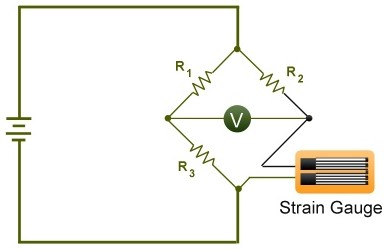
\includegraphics[width=0.6\linewidth]{Figures/Fig9}
		\caption{Wheatstone Bridge Circuit}
		\end{figure}
\end{center}
Load cells can also be used to measure the drag and lift forces.
\subsubsection{Attitude Sensor}
It is important to define the desired aerodynamic angles and to guarantee that they are measured accurately in relation to the air stream. One such angle is the angle of attack (\textalpha) shown in Figure 2.4. For this reason, specific devices that provide the attitude measurement should be implemented in order to improve the precision of the results.

Angle of attack (\textalpha)- angle measured between the longitudinal axis of the model and the direction of the flow on a vertical (Figure 2.4)
\begin{center}
	\begin{figure}[!h]
	\centering
	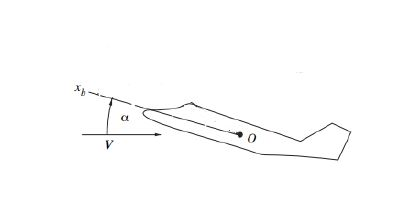
\includegraphics[width=0.6\linewidth]{Figures/Fig10}
	\caption{Angle of attack (\textalpha)}
	\end{figure}
\end{center}
\subsection{Summary of Gaps}

  \clearpage
    \section{Methodology}
\subsection{Outline}
This section will look into the mathematical designs for the Stewart platform, considerations for the force sensor and the velocity measurement within the wind tunnel. It will finally looks into the design of a human machine interface that will be used to control the Stewart platform,  obtain the measurements and display results.

\subsection{Design of Stewart Platform}
This section deals with: design considerations, position, velocity and acceleration analysis of the Stewart platform. Both kinematic analysis and dynamic analysis will be looked at.
\subsubsection{Design Considerations}
\begin{enumerate}
\item When the controllable axes are active, the platform must be controlled in six degrees of motion.
\item When the controllable members are stationary the
platform must have a corresponding fixed position.
\item The design parameters for consideration are: mobile platform radius, height of the platform and angle between adjacent joints of mobile platform and base plate.
\item The mechanism should be lightweight.
\item Velocity and position control of the mechanism should be easy to achieve.
\end{enumerate}
\subsubsection{Kinematic Analysis - Rotational matrix}
Euler angles are utilized to obtain rotational matrix for the moving platform of the Stewart platform mechanism. The rotational matrix is represented as follows \cite{csumnu2017simulation}:
\begin{equation}
 R_{P}^B = R_{Z}(\gamma)*R_{Y}(\beta)*R_{X}(\alpha)
\end{equation}
In matrix form:
\[ R_{P}^B =
 \begin{bmatrix}
 c\beta c\gamma & s\alpha s\beta c\gamma - c\alpha s\gamma & c\alpha s\beta c\gamma + s\alpha s\gamma\\
 c\beta s\gamma & s\alpha s\beta s\gamma + c\alpha c\gamma & c\alpha s\beta s\gamma - s\alpha c\gamma\\
 -s\beta & s\alpha c\beta & c\alpha c\beta  
 \end{bmatrix}
\]
Generalized coordinate position and velocity vector of the moving platform is represented below \cite{csumnu2017simulation}:
\[
q=
\begin{bmatrix}
tx & ty & tz & \alpha & \beta & \gamma
\end{bmatrix}^\top
\]
\[
\dot{q}=
\begin{bmatrix}
\dot{tx} & \dot{ty} & \dot{tz} & \dot{\alpha} & \dot{\beta} & \dot{\gamma}
\end{bmatrix}^\top
\]
Transformation of angular velocity of moving platform to the base frame can be done using Euler angles \cite{csumnu2017simulation}:
\[
\omega =
\begin{bmatrix}
1 & 0 & s\beta \\
0 & c\alpha & -s\alpha c\beta \\
0 & s\alpha & c\alpha c\beta 
\end{bmatrix}
\begin{bmatrix}
\dot{\alpha} \\
\dot{\beta}\\
\dot{\gamma}
\end{bmatrix}
\]
Acceleration of the moving platform is obtained by differentiating the velocity of the moving platform with respect to time:
\[
\dot{\omega} =
\begin{bmatrix}
1 & 0 & s\beta \\
0 & c\alpha & -s\alpha c\beta \\
0 & s\alpha & c\alpha c\alpha c\beta 
\end{bmatrix}
\begin{bmatrix}
\ddot{\alpha} \\
\ddot{\beta}\\
\ddot{\gamma}
\end{bmatrix}
+
\begin{bmatrix}
0 & 0 & \dot{\beta}c\beta \\
0 & \dot{\alpha} s\alpha & -\dot{\alpha} c\alpha c\beta + s\alpha \dot{\beta} s\beta \\
0 & \dot{\alpha}c\alpha & -\dot{\alpha}s\alpha c\beta - c\alpha \dot{\beta}s\beta
\end{bmatrix}
\begin{bmatrix}
\dot{\alpha} \\
\dot{\beta}\\
\dot{\gamma}
\end{bmatrix}
\]
\subsubsection{Inverse Kinematic Analysis}
Inverse kinematic analysis is used to determine the length of the legs according to planned trajectories of the moving platform position. In order to consider the length of the leg of a Stewart platform, closed-loop of one leg is used as shown in figure 3.1. Using this closed-form representation, the leg
vector with respect to base platform can be obtained as follows \cite{csumnu2017simulation}:
\begin{equation}
\label{eqn}
L_{i} = q_{i}^{B} - b_{i}
\end{equation}
The position vector of ith upper junction point with respect to the base frame is given by the following;
\begin{equation}
\label{eqn}
q_{i}^{B} = t + R_{p}^{B} * q_{i}^{p}
\end{equation}
\begin{center}
	\begin{figure}[!h]
	\centering
	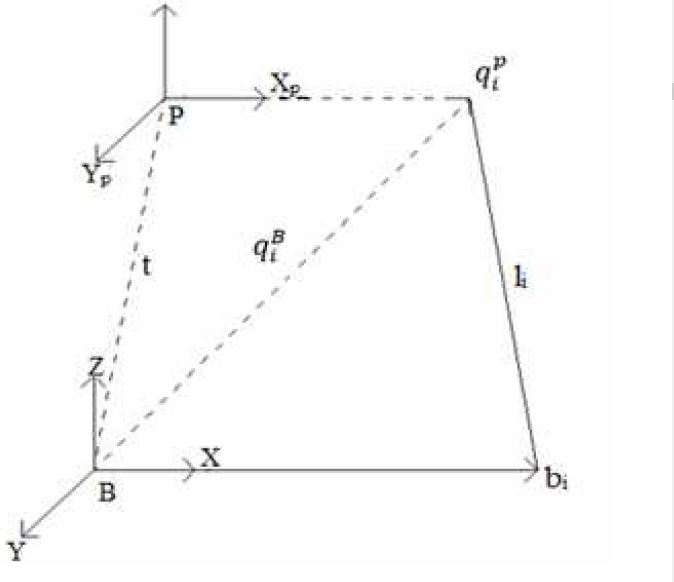
\includegraphics[width=0.6\linewidth]{Figures/Fig12}
	\caption[Closed-loop representation]{Closed-loop representation of one leg of the Stewart Platform \cite{csumnu2017simulation}}
	\end{figure}
\end{center}
Then the length of the ith leg can be acquired as follows:
\begin{equation}
\label{eqn}
l_{i}^2 = (a_{x} * r_{p} * c_{i} + b_{x}*r_{p}*s_{i} + t_{x}-r_{b}*c_{i})^2 \\+ (a_{y}*r_{p}*c_{i} + b_{y}*r_{p}*s_{i} + t_{y}-r_{b}*s_{i})^2 \\+ (a_{z}*r_{p}*c_{i}+b_{z}*r_{p}*s_{i}+t_{z})^2
\end{equation}
\subsubsection{Inverse Velocity Analysis}
Inverse Jacobian matrix can be used to perform inverse velocity analysis of the Stewart
platform. Inverse Jacobian matrix describes relation between velocity of the moving platform and the leg velocity.

Inverse Jacobian matrix for a 6-DOF Stewart Platform:
\[ J^-1 =
\begin{bmatrix}
u_{1}^{T} & (R_{P}^{B}q_{1}^{B} * u_{1})^T\\
u_{2}^{T} & (R_{P}^{B}q_{2}^{B} * u_{2})^T\\
u_{3}^{T} & (R_{P}^{B}q_{3}^{B} * u_{3})^T\\
u_{4}^{T} & (R_{P}^{B}q_{4}^{B} * u_{4})^T\\
u_{5}^{T} & (R_{P}^{B}q_{5}^{B} * u_{5})^T\\
u_{6}^{T} & (R_{P}^{B}q_{6}^{B} * u_{6})^T
\end{bmatrix}
\]
\subsubsection{PID Control of the Stewart Platform}
The controller will consist of two sections:
\begin{enumerate}
\item The leg trajectory - will be used to generate the desired leg lengths for each time step.
\item The Controller.
\end{enumerate}  The following equation will be used to calculate the leg lengths for each leg 
\cite{smith2002creating}:
\begin{equation}
\label{eqn}
((R*p_{t,i} + p)-p_{b,j}))- l_{n,i}
\end{equation}
where R is the rotation matrix relating the top plate orientation with respect to the bottom plate, $P_{t,i}$ is the attachment point of leg i in the top plate with respect to the top plate coordinate system, P is the position of the top plate with respect to the bottom plate, $P_{b,i}$ is the attachment point of leg i in the bottom plate with respect to the bottom plate coordinate system, and $ln,i$ is the nominal length of leg i. 

Proportional-integral-derivative (PID) control will be used to control the Stewart platform. A dynamic model of the system will be implemented in MatLab/Simulink.
\begin{center}
	\begin{figure}
	\centering
	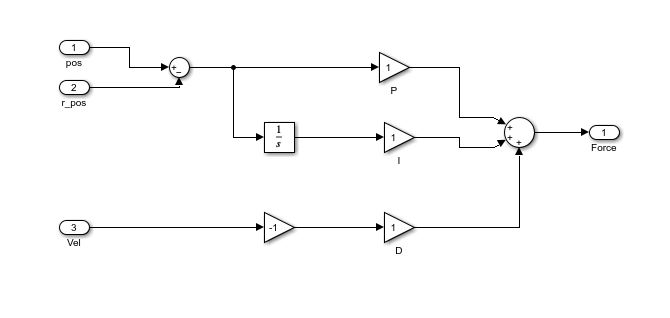
\includegraphics{Figures/Fig13}
	\caption[PID Controller]{Simple Low-level PID Controller}
	\end{figure}
\end{center}
\subsection{Design of the Force Sensor}
The force sensor module will be used to measure the force and moments from the aerodynamic loads applied on model being tested in the wind tunnel. The forces to be measured are the drag, lift and thrust as well as associated moments. For this subsystem two possible conceptual designs are to be considered:
\begin{itemize}
\item External force sensor
\item Stewart Platform as a force sensor
\end{itemize}
\subsubsection{External Force Sensor}
In this case it would require at least 3 orthogonally positioned load cells measuring each force component. Each load cell would be mechanically linked to the model such that forces experienced on each axis are measured by each load cell. 
\begin{center}
	\begin{figure}[!h]
		\centering
		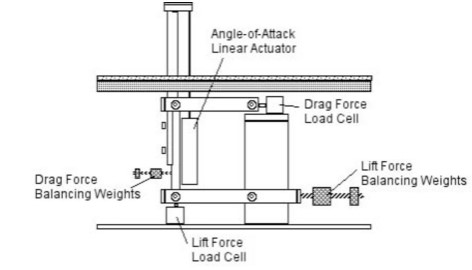
\includegraphics{Figures/modBal}
		\caption[Diagram of a force balance]{Diagram of a force balance \cite{post_force_2010}}
	\end{figure}
\end{center}
This configuration is however bulky by requiring an additional external system for force measurements in addition to the stewart platform for positioning the model. This is however complemented by the simplicity in calibration of the load cells and does not require a complex force transformation matrix and other issues with force amplification created by the use of an integrated system.
\subsubsection{Stewart Platform as a force sensor}
In this configuration the stewart platform legs are used as force sensors by attaching strain gauges in the legs of platform. Similar work has been done by \cite{ferreira2015design} without the use of actuators as is proposed in this project. Using the stewart platform as a force sensor requires the actuators to be locked with zero degrees of freedom.

Four strain gauges are required for each leg for a full wheatstone bridge configuration. 
\begin{center}
	\begin{figure}[!h]
		\centering
		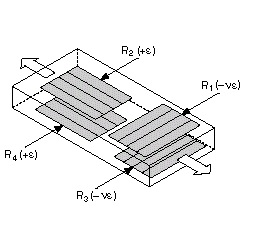
\includegraphics{Figures/loadConf}
		\caption[Strain Gauge Configuration]{Strain Gauge Configuration \cite{noauthor_measuring_nodate}}
	\end{figure}
\end{center}
In this case as shown in the figure the load cells are able to measure the axial strain on each leg. R1 and R3 are active strain gauges measuring the compressive Poisson effect (–νe). R2 and R4 are active strain gages measuring the tensile strain (+e). The output generated from the wheatstone bridge is then amplified and read to determine the strain on each leg.

\paragraph{Force measurement Circuit}
The output excitation of the wheatstone brisge needs to be amplified as it reulsts in low outputs. There is also a need to digital to analog converter. Some considerable options are the hx711 or the AD7193 converters which may be used as digital to analog converters. The AD7193 is designed for high precision and has a delta sigma filter to remove noise from measurements. 

The connection of the AD7193 to the microcontroller will be via Serial Peripheral Interface (SPI). the configuration is as shown below:
\begin{center}
\begin{figure}
\centering
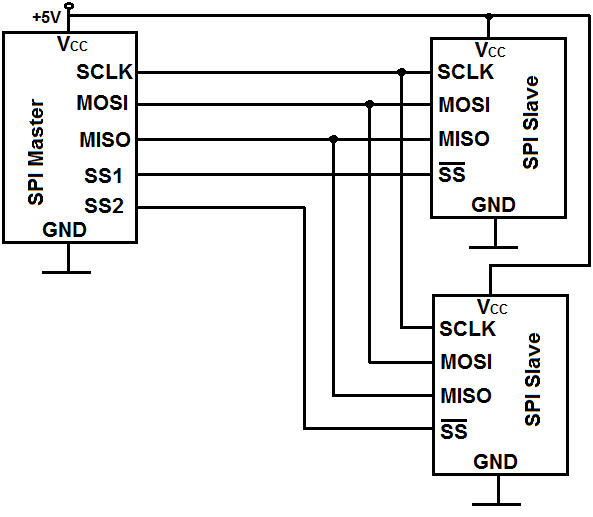
\includegraphics[width=0.55\linewidth]{Figures/SPI}
\caption[SPI configuration]{SPI configuration}
\end{figure}
\end{center}

In this configuration the when the chip select of an amplifier is set to low, the microcontroller is able to obtain data from that strain gauge. This configuration allows for a four wire interface to connect to six strain gauge sensors and obtain measurements.

\paragraph{Force transformation matrix} 
In such a case the forces experienced at the top of the platform are distributed between the 6 legs and as result, a force transformation matrix is required to resolve the forces apllied on each axis as measured by each load cell on each leg. 

If the platform is acted upon by an external wrench {$\vec{F}_e, \vec{M}_e$}, for static equilibrium of the body, the external wrench is statically balanced by the six leg forces of the stewart platform. Representing the unit vector $\hat{I}_i$ along the i-th leg with respect to B, the leg force is given  by $\hat{I}_if_i$. Considering the force equilibrium of the platform along  three mutually perpendicular directions in B(XYZ), the following force equations can be obtained as in \cite{dwarakanath_design_2001}:

$(F_e)_x = f_1I_{1x} + f_2I_{2x} + f_3I_{3x} + f_4I_{4x} + f_5I_{5x} + f_6I_{6x}$

$(F_e)_y = f_1I_{1y} + f_2I_{2y} + f_3I_{3y} + f_4I_{4y} + f_5I_{5y} + f_6I_{6y}$

$(F_e)_z = f_1I_{1z} + f_2I_{2z} + f_3I_{3z} + f_4I_{4z} + f_5I_{5z} + f_6I_{6z}$

where $(F_e)_x$, $(F_e)_y$ and $(F_e)_z$ are the external forces on the platform along three mutually perpendicular directions x, y and z of the frame B, respectively.

The moment due to the forces $\hat{I}_if_i$ about the origin of B is $(\vec{b}_i x \hat{I}_i)f_i$. Considering the moment equilibrium about x, y and z axes of B, the following moment equations can be obtained as in \cite{dwarakanath_design_2001}:

$(M_e)_x = f_1(\vec{b}_1 x \hat{I}_1)_x + f_2(\vec{b}_2 x \hat{I}_2)_x + f_3(\vec{b}_3 x \hat{I}_3)_x + f_4(\vec{b}_4 x \hat{I}_4)_x + f_5(\vec{b}_5 x \hat{I}_5)_x + f_6(\vec{b}_6 x \hat{I}_6)_x$

}$(M_e)_y = f_1(\vec{b}_1 x \hat{I}_1)_y + f_2(\vec{b}_2 x \hat{I}_2)_y + f_3(\vec{b}_3 x \hat{I}_3)_y + f_4(\vec{b}_4 x \hat{I}_4)_y + f_5(\vec{b}_5 x \hat{I}_5)_y + f_6(\vec{b}_6 x \hat{I}_6)_y$

$(M_e)_z = f_1(\vec{b}_1 x \hat{I}_1)_z + f_2(\vec{b}_2 x \hat{I}_2)_z + f_3(\vec{b}_3 x \hat{I}_3)_z + f_4(\vec{b}_4 x \hat{I}_4)_z + f_5(\vec{b}_5 x \hat{I}_5)_z + f_6(\vec{b}_6 x \hat{I}_6)_z$

where $(M_e)_x$, $(M_e)_y$ and $(M_e)_z$ are the external moments on the platform  about the three coordinate axes of B. Combining the equations the relationship between the external wrench and the forces experienced by the legs can be expressed as follows:
$$
\begin{Bmatrix}
\vec{F}_e \\
\vec{M}_e \\
\end{Bmatrix} = [H]\{F\}
$$

\subsection{Velocity Measurement}
An important part in wind tunnel measurements is the measure of pressure at specific points in the wind tunnel and computing the corresponding air speed. This is achieved by the use of a pitot probe. 
\begin{center}
\begin{figure}
\centering
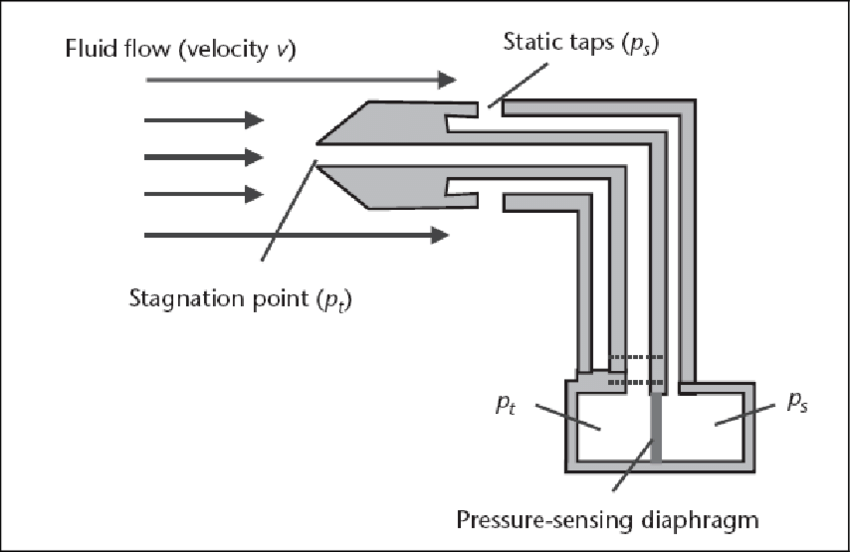
\includegraphics[width=0.7\linewidth]{Figures/pitot}
\caption[Pitot-static tube]{Pitot-static tube \cite{viquerat2006continuous}}
\end{figure}
\end{center}

The equation relates the speed of the fluid at a point to both the mass density of the fluid and the pressures at the same point in the flow field. For steady flow of an incompressible fluid for which viscosity can be neglected, the fundamental equation has the form:

$$ v = \sqrt{\frac{2(P_0 - P)}{\rho}}$$

Where V is the speed of the fluid, P0 is the total, also called the stagnation, pressure at that point of measurement, and p is the static pressure at the same point.

Three pitot probes are to be used in the wind tunnel, these are in the test section, intake and dissuser sections.

\subsection{Design of Human Machine Interface}
The purpose of the interface is to enable control of the platform position as well as to obtain measured data from the strain gauges and pitot tubes. 
The general layout is as shown in the figure below:
\begin{center}
\begin{figure}
\centering
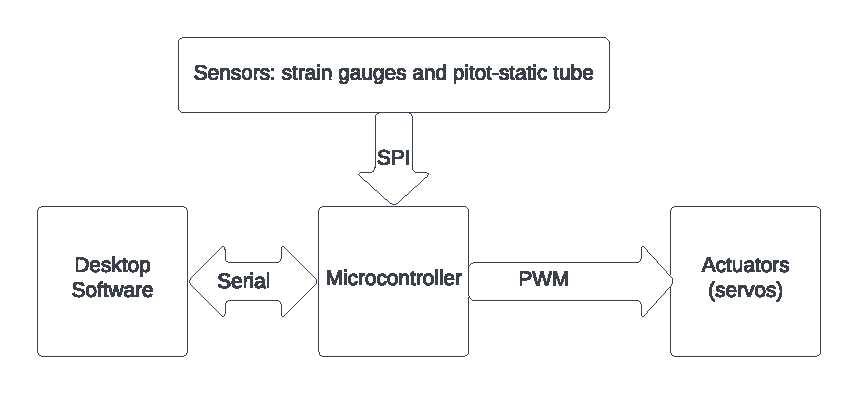
\includegraphics{Figures/interface}
\caption[Human Machine Interface]{Human Machine Interface}
\end{figure}
\end{center}

The primary interface between the microcontroller is via serial interface by use of USB. This is used due to wide availability and integration on many personal computers. Serial communication allows for bidirectional transfer of information thus allowing for both control input and output of measured values. The interface is to enable the abstraction of data aquisition and actuator control to a simple interaction with buttons and other visual interfaces available in a computer program.

The decoupling of the microcontroller and the program to be hosted on the desktop allows for advanced data processing such as application of filters and resolving measurements into useable information. It also allows for the use of more powerful processor and high level programmming languages to more effectively perform complex calculations without taking a toll the sensor samping rate that would occur with onboard processing in the microcontroller.
\newpage
\begin{center}
	\begin{figure}[!h]
	\centering
	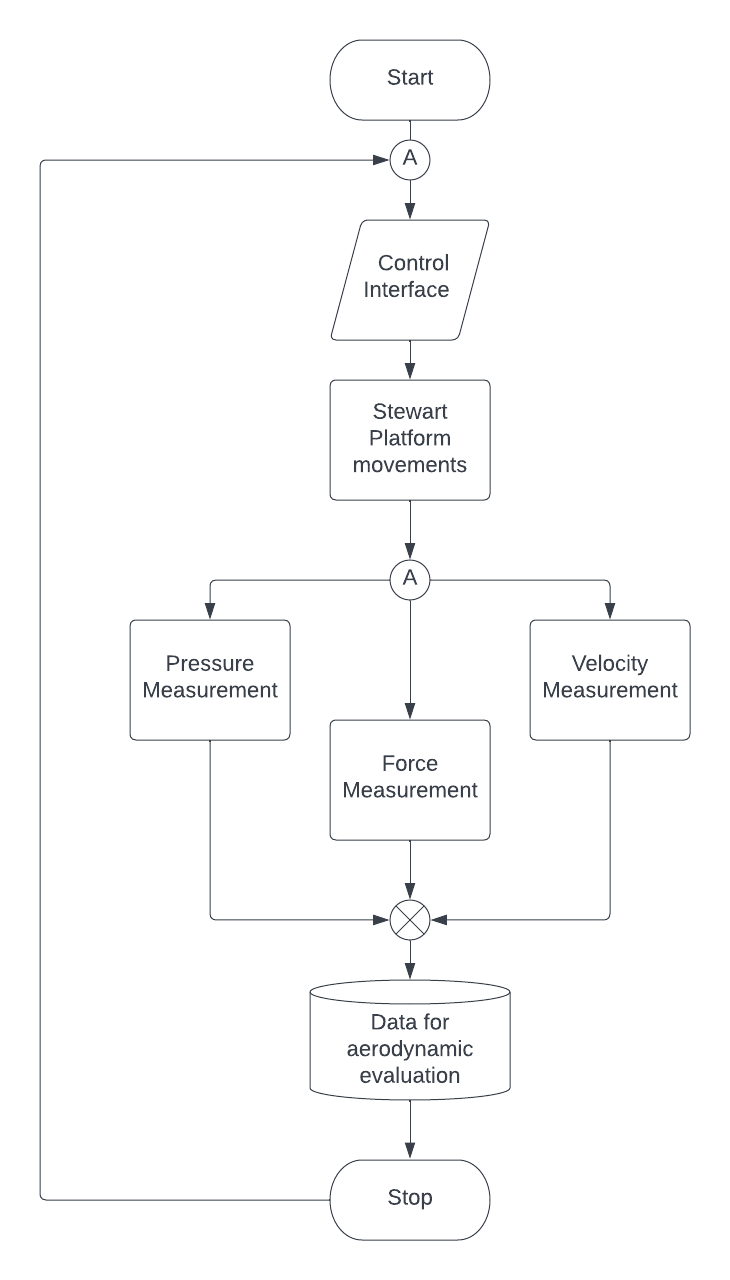
\includegraphics[width=0.7\linewidth]{Figures/Fig14}
	\caption[Control Algorithim]{Control Algorithim for the Stewart Platform with Force Measurement}
	\end{figure}
\end{center}
  \clearpage
    \section{Expected Outcomes}
\begin{enumerate}
\item A fuctional stewart platform with six degrees of freedom postioning of a model within a wind tunnel.
\item A functional force sensor for measuring the aerodynamic load applied on a model and calculate aerodynamic coefficients from the meaurements taken.
\item An improved velocity measurement system for the wind tunnel using pitot tubes.
\item A human Machine Interface with access to control  of the stewaart platform electronics and data aquisition from sensors.
\end{enumerate}
\newpage
\subsection{Proposed Budget}
\begin{center}
\begin{table}[!h]
\centering
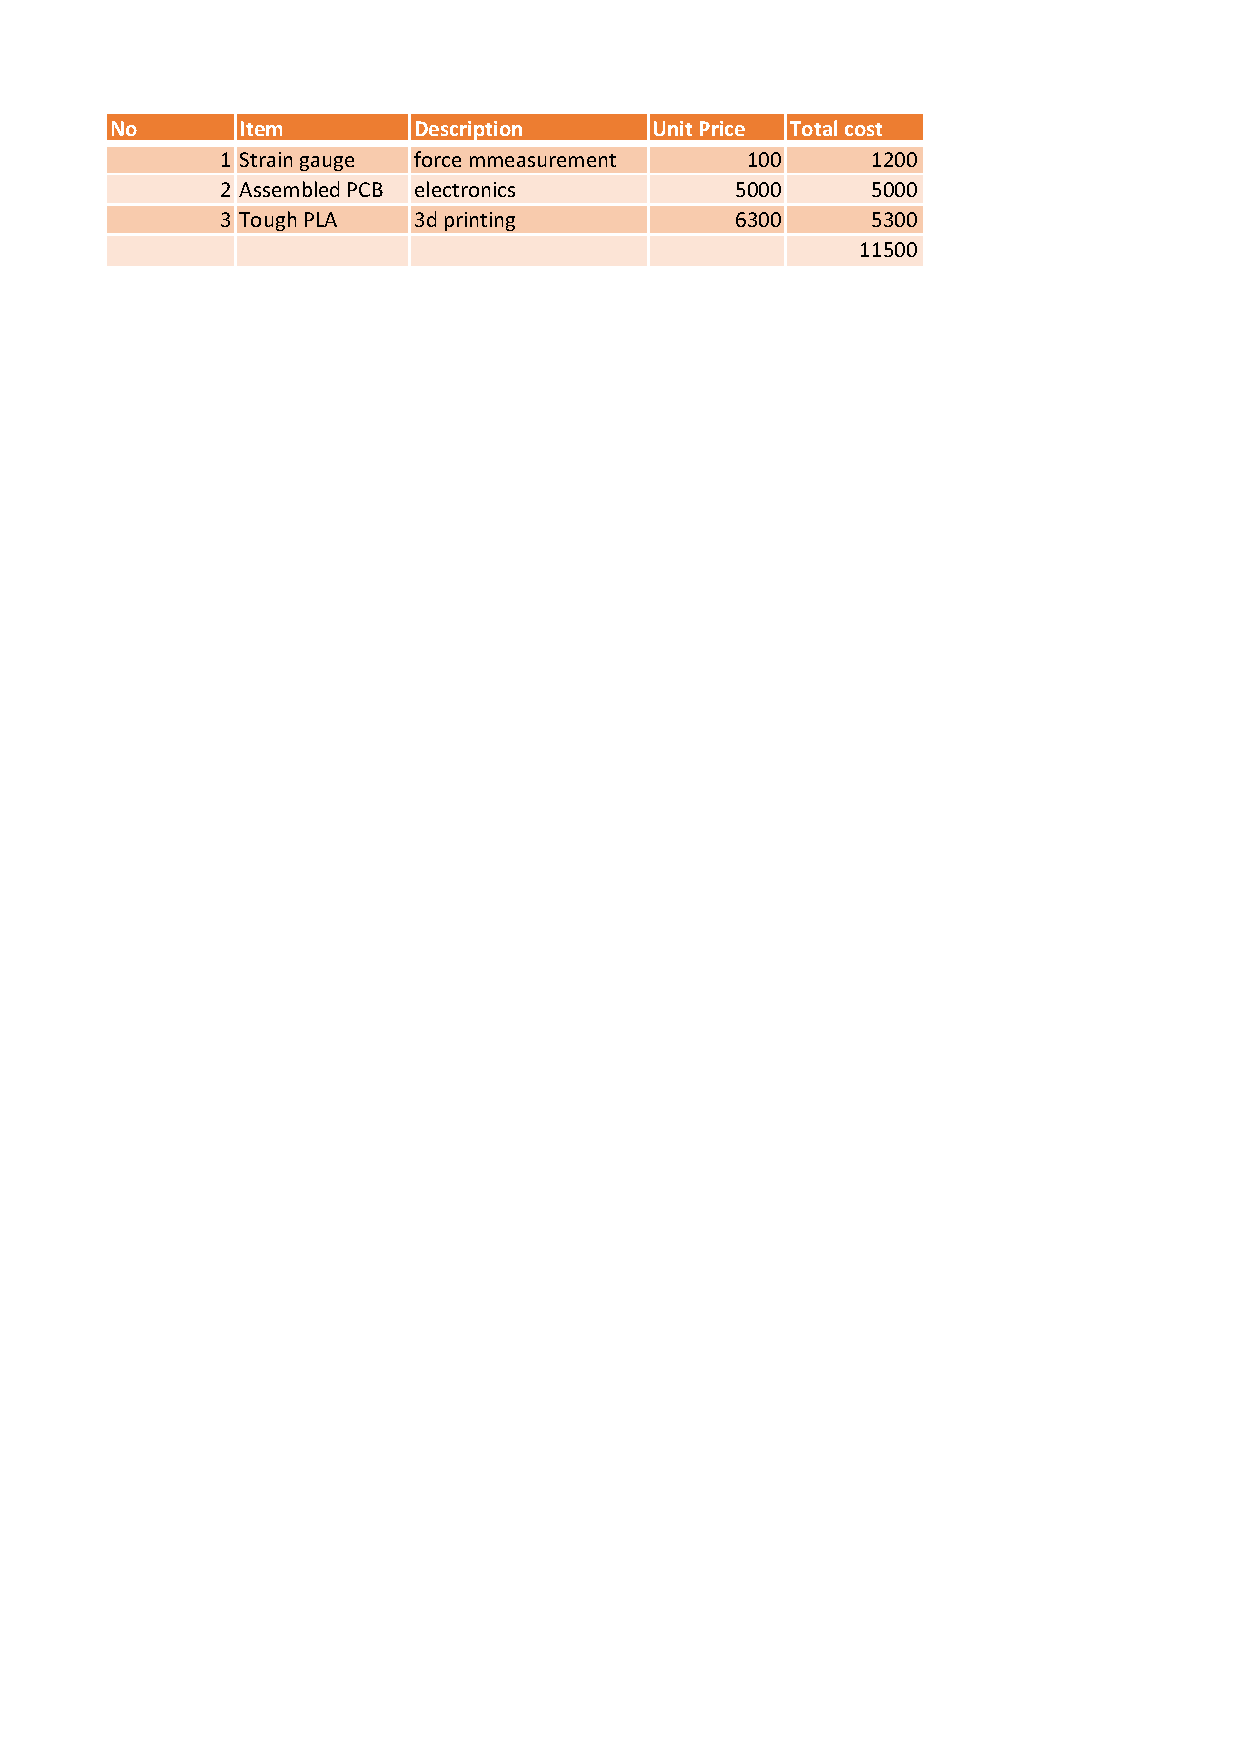
\includegraphics{Figures/budget}
\caption{Proposed budget}
\end{table}
\end{center}
\subsection{Work Plan}
\begin{center}
\begin{table}[!h]
\centering
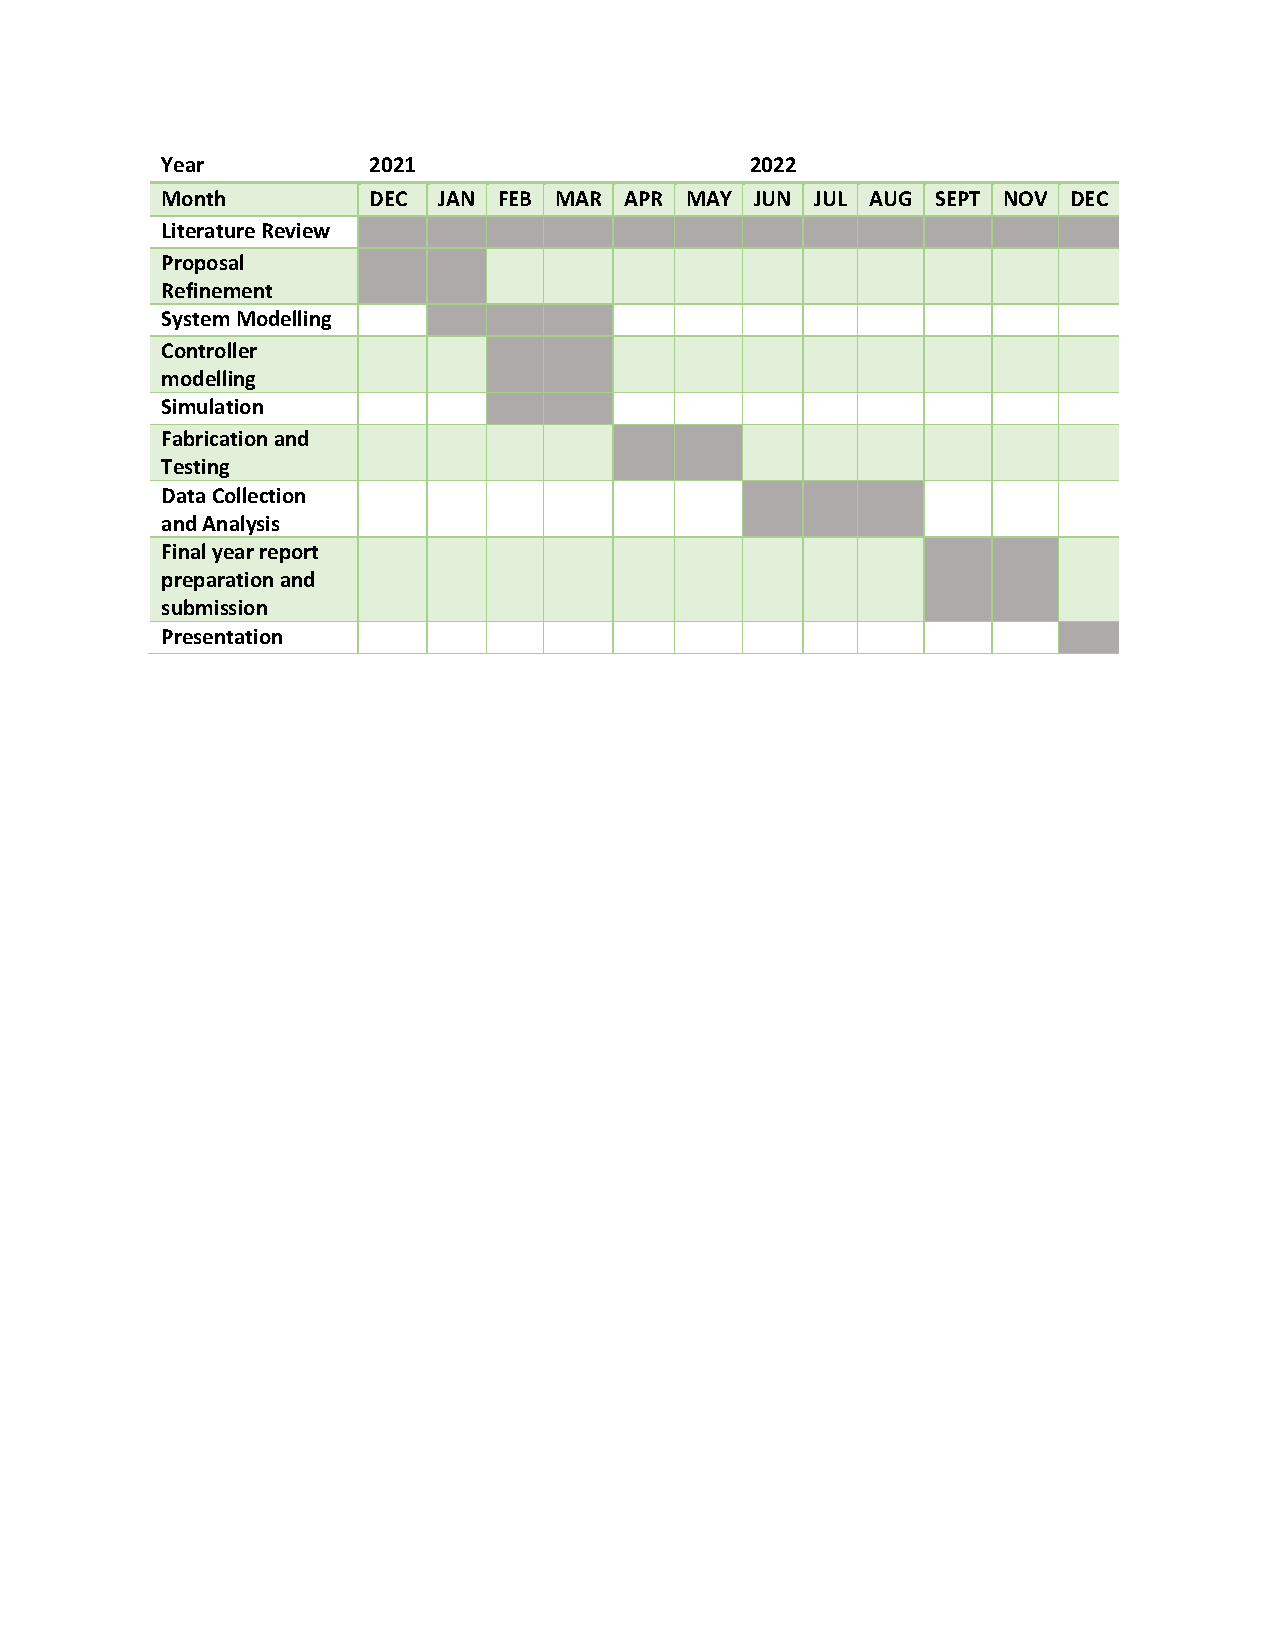
\includegraphics[width=0.95\linewidth]{Figures/workplan}
\caption{Workplan table}
\end{table}
\end{center}

%  \clearpage
%  \section{Appendices}
  \clearpage
%----  Bibliography  ----------------------------------------
\markright{References}                               % Erzeugt Kopfzeile
\addcontentsline{toc}{section}{References}            % Literaturverzeichnis ins Inhaltsverzeichnis
\bibliographystyle{Bib/IEEEtran}
\bibliography{Bib/References}                         % BIBTeX
\nocite{Lun01} 

                                     % Falls etwas in die Literaturliste soll, was nicht Referenziert wird
\end{document}
